\subsection{Parametrické vyjádření přímky}
\label{subsec:Parametric_line}

Parametrické vyjádření přímky je založeno na myšlence,
že přímka může být popsána pomocí bodu, kterým prochází, a směru, kterým se táhne.
Toto vyjádření je velmi intuitivní a často se používá v praxi,
zejména v počítačové grafice a fyzice.

\begin{remark}
    V počítačové grafice se parametrické vyjádření přímky často používá k 
    interpolaci mezi dvěma body nebo k popisu trajektorie pohybu.
    Ve fyzice se zase využívá k popisu pohybu částic nebo k modelování silových polí.
\end{remark}

Protože víme, že přímka je určitý druh čáry, rovné čáry, která 
nemá žádné zakřivení a táhne se nekonečně daleko v obou směrech.
A protože již víme, že pomocí vektoru můžeme popsat směr a zároveň
se můžeme díky násobkům vektoru posouvat dále, či blíže od počátečního bodu,
můžeme přímku popsat pomocí směrového vektoru a bodu, kterým prochází.

\begin{definition}\label{def:Parametric_line}
    Nechť $A$ je bod v rovině a $\vec{u}$ je nenulový vektor.
    Pak přímka $p$ procházející bodem $A$ a směrem určeným směrovým vektorem $\vec{u}$ může být vyjádřena jako množina všech bodů $X$, které lze získat jako
    \begin{equation}
        X = A + t\vec{u}, \quad t \in \mathbb{R}.
    \end{equation}
    Rozšířením této rovnice do souřadnic získáme parametrické rovnice přímky:
    \begin{equation}
        \begin{aligned}
            x &= x_A + t u_x, \\
            y &= y_A + t u_y,
            \qquad t \in \mathbb{R}.
        \end{aligned}
        \label{eq:Parametric_line_coordinate_form}
    \end{equation}
    kde $A[x_A; y_A]$ jsou souřadnice bodu $A$ a $\vec{u} = (u_x; u_y)$ jsou souřadnice směrového vektoru $\vec{u}$.

    Tento způsob vyjádření přímky se nazývá \textbf{parametrické vyjádření přímky}.
\end{definition}

V tomto vyjádření je $t$ nazýván \textbf{parametrem} přímky.
Mění-li se $t$, mění se i bod $X$ na přímce, a tím pádem můžeme získat všechny body na přímce.
Pro $t=0$ získáme bod $A$, který jsme zvolili jako jeden pevný bod přímky.
Přímka sama nemá žádný počáteční ani koncový bod, protože se neomezeně
rozprostírá v obou směrech.
Když $t$ je kladné, získáme body na přímce ve směru vektoru $\vec{u}$, a když $t$ je záporné, získáme body na přímce v opačném směru.

\begin{figure}[H]
    \centering
    \begin{tikzpicture}[scale=1]

        % Bod A
        \coordinate (A) at (1,2);
        \fill (A) circle (2pt) node[right] {$A[1,2]$};

        % Směrový vektor
        \coordinate (U) at (3,4);
        \draw[vector] (A) -- (U) node[midway, above left] {$\vec{u}$};

        % Přímka (prodloužení směru)
        \draw[thin] (-1,0) -- (5,6) node[right] {$p$};

    \end{tikzpicture}
    \caption{Parametrické vyjádření přímky $p$ dané bodem $A$ a vektorem $\vec{u}$.}
    \label{fig:Parametric_line}
\end{figure}

\begin{remark}
    Směrový vektor přímky není určen jednoznačně. Je-li $\vec{u}$
    směrovým vektorem přímky, potom je jejím směrovým vektorem také
    každý jeho nenulový reálný násobek
    \[
        k\cdot\vec{u},\qquad k\in\mathbb{R}\setminus\{0\}.
    \]
    Všechny tyto vektory jsou navzájem rovnoběžné, a určují proto
    stejný směr přímky.
\end{remark}

Z této skutečnosti zároveň plyne, že ani parametrické vyjádření přímky
není jednoznačné. Pro tutéž přímku můžeme zvolit kterýkoli její bod
a kterýkoli nenulový směrový vektor rovnoběžný s přímkou.

Například zápisy
\begin{align*}
    p: x &= 1+2t,\\
       y &= 2+2t;\quad t\in\mathbb{R},
\end{align*}
a
\begin{align*}
    p: x &= 3-4s,\\
       y &= 4-4s;\quad s\in\mathbb{R}
\end{align*}
popisují tutéž přímku. Druhý zápis totiž používá bod $[3;4]$, který
na původní přímce leží, a směrový vektor $(-4;-4)$, jenž je násobkem
původního směrového vektoru $(2;2)$.

\begin{example}
    Mějme bod $A[1; 2]$ a vektor $\vec{u} = (2; 2)$.
    Najděme parametrické vyjádření přímky $p$, která prochází bodem $A$ a má směr určený vektorem $\vec{u}$.

    Podle definice \ref{def:Parametric_line} můžeme přímku $p$ vyjádřit jako
    \begin{align*}
        X   &= A + t\vec{u} \\
            &= [1; 2] + t(2; 2) \\
            &= [1 + 2t; 2 + 2t], \quad t \in \mathbb{R}.
    \end{align*}

    Což můžeme zapsat následujícími způsoby:
    \begin{align*}
        p:  x &= 1 + 2t, \\
            y &= 2 + 2t; \quad t \in \mathbb{R}.
    \end{align*}

    Případně můžeme využít zápis pomocí množin:
    \[
        p = \{ [x; y] \in \mathbb{R}^2 \mid x = 1 + 2t, y = 2 + 2t, t \in \mathbb{R} \},
    \]
    nebo:
    \[
        p = \{ [1 + 2t; 2 + 2t] ; t \in \mathbb{R} \}.
    \]

    Všechny tři způsoby zápisu jsou ekvivalentní a popisují stejnou přímku $p$ v rovině.
\end{example}

\begin{example}
    Mějme parametrické vyjádření přímky $q$ dané jako:
    \begin{align*}
        q:  x &= 3 + 4t, \\
            y &= 1 - t; \quad t \in \mathbb{R}.
    \end{align*}
    Najděme bod, kterým přímka $q$ prochází, a vektor, který určuje její směr.

    Z parametrického vyjádření přímky $q$ můžeme snadno určit bod, kterým prochází, a vektor, který určuje její směr.
    Bod $B$ je dán hodnotami $x$ a $y$ pro $t=0$:
    \[
        B = [3 + 4 \cdot 0; 1 - 0] = [3; 1].
    \]
    Souřadnice jednoho bodu přímky tedy získáme z konstantních členů parametrických rovnic, zatímco souřadnice směrového vektoru tvoří koeficienty u parametru $t$.
    Vektor $\vec{v}$, který určuje směr přímky $q$, je dán koeficienty u $t$ v rovnicích pro $x$ a $y$:
    \[
        \vec{v} = (4; -1).
    \]
    Můžeme tedy opět rovnou určit vektor $\vec{v}$ tak, že vezmeme koeficienty u $t$ z obou rovnic.
    
    Tedy přímka $q$ prochází bodem $B[3; 1]$ a má směr určený vektorem $\vec{v} = (4; -1)$.
\end{example}

\begin{example}
    Zjistěte hodnoty dalších bodů na přímce $p$ z prvního příkladu pro různé hodnoty parametru $t$.
    \begin{align*}
        p : x &= 1 + 2t, \\
            y &= 2 + 2t; \quad t \in \mathbb{R}.
    \end{align*}

    Pro zjištění dalších bodů na přímce $p$ můžeme dosadit různé hodnoty parametru $t$ do rovnic pro $x$ a $y$,
    a získat tak souřadnice dalších bodů na přímce.

    Pro $t = 1$:
    \begin{align*}
        x &= 1 + 2 \cdot 1 = 3, \\
        y &= 2 + 2 \cdot 1 = 4.
    \end{align*}
    Tedy bod $C$ na přímce $p$ pro $t=1$ je $C[3; 4]$.

    Pro $t = -1$:
    \begin{align*}
        x &= 1 + 2 \cdot (-1) = -1, \\
        y &= 2 + 2 \cdot (-1) = 0.
    \end{align*}
    Tedy bod $D$ na přímce $p$ pro $t=-1$ je $D[-1; 0]$.

    Pro $t = 0.5$:
    \begin{align*}
        x &= 1 + 2 \cdot \tfrac{1}{2} = 2, \\
        y &= 2 + 2 \cdot \tfrac{1}{2} = 3.
    \end{align*}
    Tedy bod $E$ na přímce $p$ pro $t=\frac{1}{2}$ je $E[2; 3]$.
\end{example}

\begin{example}\label{exa:Points_on_parametric_line}
    Zjistěte, zda-li body $F[5; 6]$ a $G[0; 0]$ leží na přímce $p$, která je dána parametrickým vyjádřením:
    \begin{align*}
        p : x &= 1 + 2t, \\
            y &= 2 + 2t; \quad t \in \mathbb{R}.
    \end{align*}

    Pro zjištění, zda-li bod $F[5; 6]$ leží na přímce $p$, musíme zjistit, zda existuje hodnota parametru $t$, pro kterou platí rovnice pro $x$ a $y$.
    Dosadíme tedy souřadnice bodu $F$ do rovnic pro $x$ a $y$ a zjistíme, zda-li existuje společné řešení pro $t$.

    \begin{align*}
        5 &= 1 + 2t \quad \Rightarrow \quad 2t = 4 \quad \Rightarrow \quad t = 2, \\
        6 &= 2 + 2t \quad \Rightarrow \quad 2t = 4 \quad \Rightarrow \quad t = 2.
    \end{align*}

    Pro $t=2$ platí obě rovnice, tedy bod $F[5; 6]$ leží na přímce $p$.

    Pro zjištění, zda-li bod $G[0; 0]$ leží na přímce $p$, opět dosadíme souřadnice bodu $G$ do rovnic pro $x$ a $y$ a zjistíme, zda-li existuje společné řešení pro $t$.
    \begin{align*}
        0 &= 1 + 2t \quad \Rightarrow \quad 2t = -1 \quad \Rightarrow \quad t = -\frac{1}{2}, \\
        0 &= 2 + 2t \quad \Rightarrow \quad 2t = -2 \quad \Rightarrow \quad t = -1.
    \end{align*}
    Pro $x$ a $y$ získáváme různé hodnoty pro $t$, tedy neexistuje žádná hodnota parametru $t$, pro kterou by platily obě rovnice, a proto bod $G[0; 0]$ neleží na přímce $p$.

\end{example}

V příkladu \ref{exa:Points_on_parametric_line} jsme zjistili, že bod
$F[5;6]$ na přímce $p$ leží, protože pro obě jeho souřadnice vyšla
stejná hodnota parametru $t=2$. Naopak pro bod $G[0;0]$ jsme z první
rovnice získali $t=-\frac12$, zatímco z druhé rovnice $t=-1$.
Neexistuje tedy jediná hodnota parametru, která by současně vytvořila
obě souřadnice bodu $G$.

Stejnou skutečnost můžeme vysvětlit také pomocí vektorů. Vektor směřující
z bodu $A[1;2]$ do bodu $G[0;0]$ je
\[
    \overrightarrow{AG}=(0-1;0-2)=(-1;-2).
\]
Aby bod $G$ ležel na přímce $p$, musel by být vektor
$\overrightarrow{AG}$ reálným násobkem směrového vektoru
$\vec{u}=(2;2)$. To však neplatí, protože neexistuje číslo
$k\in\mathbb{R}$, pro které by současně platilo
\[
    (-1;-2)=k(2;2).
\]
Vektory $\overrightarrow{AG}$ a $\vec{u}$ nejsou rovnoběžné, a proto
bod $G$ na přímce $p$ neleží.

\begin{figure}[H]
    \centering
    \begin{tikzpicture}[scale=0.8]

        % Body
        \coordinate (A) at (1,2);
        \coordinate (F) at (5,6);
        \coordinate (G) at (0,0);

        \fill (A) circle (2pt) node[right] {$A[1; 2]$};
        \fill (F) circle (2pt) node[right] {$F[5; 6]$};
        \fill (G) circle (2pt) node[left] {$G[0; 0]$};

        % Směrový vektor u
        \coordinate (U) at (3,4);
        \draw[vector] (A) -- (U) node[midway, above left] {$\vec{u}$};

        % Vektor k bodu G (není rovnoběžný)
        \draw[vector, dashed] (A) -- (G) node[midway, below] {$\vec{v}$};

        % Přímka
        \draw[thin] (0,1) -- (6,7) node[right] {$p$};

    \end{tikzpicture}
    \caption{Bod $F$ leží na přímce $p$, zatímco bod $G$ neleží na přímce $p$.}
    \label{fig:Parametric_line_points}
\end{figure}

Zatím jsme přímku v rovině ještě neurčovali, ale zasipovali jsme ji pomocí bodu a směrového vektoru.
Jak jsme si ukázali, tak bod na přímce je dán souřadnicemi, které získáme dosazením hodnot za parametry (násobky směrového vektoru) do parametrické rovnice přímky.
Tedy pokud chceme přímku v rovině určit, tak potřebujeme bod a směrový vektor, který určuje směr přímky (viz definice \ref{def:Parametric_line}).
Můžeme tedy dopočítat i parametrické vyjádření přímky, pokud máme dva body, které na přímce leží.

V dosavadních příkladech jsme znali bod přímky a její směrový vektor. Často jsou však zadány dva různé body $A[x_A;y_A]$ a $B[x_B;y_B]$, kterými má přímka procházet. Protože dvěma různými body v rovině prochází právě jedna přímka, získáme její směrový vektor jako
\[
    \overrightarrow{AB}=(x_B-x_A;y_B-y_A).
\]
Parametrické vyjádření potom můžeme sestavit ve tvaru
\begin{equation}\label{eq:Parametric_line_two_points}
    X=A+t\overrightarrow{AB},\qquad t\in\mathbb{R},
\end{equation}

Geometrický význam vztahu \eqref{eq:Parametric_line_two_points}
je znázorněn na obrázku \ref{fig:Parametric_line_two_points}.
Z bodu $A$ se pomocí různých reálných násobků vektoru
$\overrightarrow{AB}$ můžeme pohybovat po celé přímce v obou směrech.

\begin{figure}[H]
    \centering
    \begin{tikzpicture}[scale=1]

        % Body
        \coordinate (A) at (0,0);
        \coordinate (B) at (3,2);

        % Přímka
        \draw[thin] (-1,-0.67) -- (5,3.33) node[right] {$p$};

        % Body A a B
        \fill (A) circle (2pt) node[below right] {$A$};
        \fill (B) circle (2pt) node[below right] {$B$};

        % Směrový vektor
        \draw[vector] (A) -- (B)
            node[midway, above left] {$\overrightarrow{AB}$};

    \end{tikzpicture}
    \caption{Přímka $p$ určená dvěma různými body $A$ a $B$ a směrovým vektorem $\overrightarrow{AB}$.}
    \label{fig:Parametric_line_two_points}
\end{figure}

Parametrické rovnice přímky tedy po rozepsání souřadnic znamená
\begin{align}
    x &= x_A+t(x_B-x_A),\\
    y &= y_A+t(y_B-y_A);\quad t\in\mathbb{R}.
\end{align}

Můžeme tedy upravit definici \ref{def:Parametric_line} tak, že přímku určíme dvěma body, kterými prochází.
\begin{definition}
    Nechť $A$ a $B$ jsou dva různé body v rovině. Pak přímka $p$ procházející body $A$ a $B$ může být vyjádřena jako množina všech bodů $X$, které lze získat jako
    \begin{equation}
        X = A + t\overrightarrow{AB}, \quad t \in \mathbb{R}.
    \end{equation}
    Rozšířením této rovnice do souřadnic získáme parametrické rovnice přímky:
    \begin{equation}
        \begin{aligned}
            x &= x_A + t(x_B - x_A), \\
            y &= y_A + t(y_B - y_A),
            \qquad t \in \mathbb{R}.
        \end{aligned}
        \label{eq:Parametric_line_two_points_coordinate_form}
    \end{equation}
    Tento způsob vyjádření přímky se nazývá \textbf{parametrické vyjádření přímky určené dvěma body}.
\end{definition}


\begin{example}\label{exa:Parametric_line_from_two_points}
    Mějte dva body $H[2; 3]$ a $I[5; 7]$.
    Najděte parametrické vyjádření přímky $r$, která prochází těmito dvěma body.

    Nejprve určíme směrový vektor $\vec{w}$ přímky $r$ jako vektor směřující z bodu $H$ do bodu $I$:
    \[
        \vec{w} = \overrightarrow{HI} = (5 - 2; 7 - 3) = (3; 4).
    \]

    Nyní můžeme použít bod $H$ a směrový vektor $\vec{w}$ k vytvoření parametrického vyjádření přímky $r$:
    \begin{align*}
        r: x &= 2 + 3t, \\
           y &= 3 + 4t; \quad t \in \mathbb{R}.
    \end{align*}

    Tedy parametrické vyjádření přímky $r$, která prochází body $H[2; 3]$ a $I[5; 7]$, je dáno výše uvedenými rovnicemi.
    Geometrický princip tohoto postupu je znázorněn na obrázku \ref{fig:Parametric_line_two_points}.
\end{example}

Zatím jsme řešili pouze přímky v rovině, ale pomocí změny hodnot parametru $t$ můžeme získat i jiné rovinné útvary, například \textbf{úsečky} a \textbf{polopřímky}.
Využijeme příklad \ref{exa:Parametric_line_from_two_points}, kde jsme získali parametrické vyjádření přímky $r$ procházející body $H[2; 3]$ a $I[5; 7]$.

\begin{example}\label{exa:Parametric_ray_through_two_points}
    Určete parametrické vyjádření polopřímky $\overrightarrow{HI}$
    z příkladu \ref{exa:Parametric_line_from_two_points}, která začíná
    bodem $H$ a prochází bodem $I$.

    Polopřímka $\overrightarrow{HI}$ začíná v bodě $H$ a pokračuje
    neomezeně daleko ve směru bodu $I$. Nejprve určíme vektor
    \[
        \overrightarrow{HI}
        =(5-2;7-3)
        =(3;4).
    \]

    Použijeme-li bod $H[2;3]$ a směrový vektor
    $\overrightarrow{HI}=(3;4)$, získáme parametrické vyjádření
    přímky procházející body $H$ a $I$:
    \begin{align*}
        r: x &= 2+3t,\\
           y &= 3+4t;\quad t\in\mathbb{R}.
    \end{align*}

    Chceme-li však popsat pouze polopřímku $\overrightarrow{HI}$,
    musíme parametr omezit na nezáporné hodnoty. Pro $t=0$ získáme
    počáteční bod $H$, pro $t=1$ bod $I$ a pro $t>1$ body ležící
    za bodem $I$ ve stejném směru.

    První parametrické vyjádření polopřímky tedy je
    \begin{align*}
        r_1: x &= 2+3t,\\
             y &= 3+4t;
             \quad t\in\langle 0;+\infty).
    \end{align*}

    Tutéž polopřímku můžeme popsat také pomocí opačně orientovaného
    vektoru
    \[
        \overrightarrow{IH}
        =(2-5;3-7)
        =(-3;-4).
    \]

    V tomto případě je vhodné použít jako pevný bod bod $I[5;7]$.
    Dostáváme tedy
    \begin{align*}
        r_2: x &= 5-3t,\\
             y &= 7-4t.
    \end{align*}

    Pro $t=1$ získáme bod
    \[
        [5-3;7-4]=[2;3]=H,
    \]
    zatímco pro $t=0$ získáme bod $I$. Abychom získali také všechny
    body ležící za bodem $I$ ve směru polopřímky $\overrightarrow{HI}$,
    musíme připustit všechny hodnoty $t\leq 1$.

    Druhé parametrické vyjádření téže polopřímky proto je
    \begin{align*}
        r_2: x &= 5-3t,\\
             y &= 7-4t;
             \quad t\in(-\infty;1\rangle.
    \end{align*}

    Geometrické znázornění polopřímky $\overrightarrow{HI}$ je uvedeno na obrázku \ref{fig:Parametric_ray_HI}. 
    Je na něm patrné, že bod $H$ je počátečním bodem polopřímky, zatímco bod $I$ určuje směr jejího dalšího pokračování.
\end{example}

\begin{figure}[H]
    \centering
    \begin{tikzpicture}[scale=0.65]

        % Body polopřímky
        \coordinate (H) at (2,3);
        \coordinate (I) at (5,7);
        \coordinate (R) at (7.25,10);

        % Polopřímka
        \draw[thin, ->] (H) -- (R);

        % Body H a I
        \fill (H) circle (2.5pt) node[below right] {$H[2;3]$};
        \fill (I) circle (2.5pt) node[below right] {$I[5;7]$};

        % Směrový vektor
        \draw[vector] (H) -- (I)
            node[midway, above, sloped] {$\vec{w}$};

        % Označení pokračování
        \node[below right] at (R) {$\overrightarrow{HI}$};

    \end{tikzpicture}
    \caption{Polopřímka $\overrightarrow{HI}$ začíná v bodě $H$, prochází bodem $I$ a pokračuje neomezeně daleko ve směru bodu $I$}
    \label{fig:Parametric_ray_HI}
\end{figure}

Oba zápisy z příkladu
\ref{exa:Parametric_ray_through_two_points} popisují tutéž polopřímku
$\overrightarrow{HI}$, přestože používají jiný pevný bod, opačně
orientované směrové vektory a jiný obor hodnot parametru.

Ekvivalenci obou zápisů můžeme ověřit substitucí
\[
    s=1-t.
\]
Protože ve druhém zápisu platí $t\leq 1$, dostáváme
\[
    s\geq 0.
\]

Dosadíme-li $t=1-s$ do druhého parametrického vyjádření, získáme
\begin{align*}
    x &= 5-3(1-s)
       =5-3+3s
       =2+3s,\\
    y &= 7-4(1-s)
       =7-4+4s
       =3+4s.
\end{align*}

Tedy
\begin{align*}
    x &= 2+3s,\\
    y &= 3+4s;
    \quad s\in\langle0;+\infty),
\end{align*}
což je právě první parametrické vyjádření polopřímky
$\overrightarrow{HI}$.


Nyní se zaměříme na úsečku $\overline{HI}$. Zatímco přímka procházející
body $H$ a $I$ pokračuje neomezeně daleko v obou směrech a polopřímka
$\overrightarrow{HI}$ pokračuje neomezeně daleko pouze ve směru od bodu
$H$ přes bod $I$, úsečka obsahuje pouze body ležící mezi body $H$ a $I$,
včetně obou jejích krajních bodů.

Protože při parametrickém vyjádření
\[
    X=H+t\overrightarrow{HI}
\]
odpovídá hodnotě $t=0$ bod $H$ a hodnotě $t=1$ bod $I$, získáme právě
úsečku $\overline{HI}$ omezením parametru na uzavřený interval
$\langle0;1\rangle$.

\begin{example}\label{exa:Parametric_segment_between_two_points}
    Určete parametrické vyjádření úsečky $\overline{HI}$ z příkladu
    \ref{exa:Parametric_line_from_two_points}, jejíž krajní body jsou
    \[
        H[2;3],\qquad I[5;7].
    \]

    Nejprve připomeňme, že vektor směřující z bodu $H$ do bodu $I$ je
    \[
        \overrightarrow{HI}
        =(5-2;7-3)
        =(3;4).
    \]

    Použijeme-li bod $H[2;3]$ a vektor $\overrightarrow{HI}=(3;4)$,
    dostáváme parametrické vyjádření přímky
    \begin{align*}
        x &= 2+3t,\\
        y &= 3+4t.
    \end{align*}

    Abychom získali pouze body úsečky $\overline{HI}$, omezíme parametr
    na interval
    \[
        t\in\langle0;1\rangle.
    \]

    Parametrické vyjádření úsečky je tedy
    \begin{align*}
        \overline{HI}: x &= 2+3t,\\
                         y &= 3+4t,
                         \qquad t\in\langle0;1\rangle.
    \end{align*}

    Pro $t=0$ získáme bod
    \[
        [2+3\cdot0;3+4\cdot0]=[2;3]=H,
    \]
    zatímco pro $t=1$ získáme bod
    \[
        [2+3\cdot1;3+4\cdot1]=[5;7]=I.
    \]

    Hodnoty parametru $0<t<1$ určují body ležící uvnitř úsečky.
    Například pro $t=\frac12$ dostáváme
    \[
        \left[
            2+3\cdot\frac12;
            3+4\cdot\frac12
        \right]
        =
        \left[
            \frac72;5
        \right],
    \]
    což je střed úsečky $\overline{HI}$. Což můžeme ověřit také dosazením do vzorce (viz vzorec z definice \ref{def:midpoint}):
    \[
        S=\left[
            \frac{2+5}{2};
            \frac{3+7}{2}
        \right]
        =
        \left[
            \frac72;5
        \right].
    \]

    Úsečka $\overline{HI}$ a její střed odpovídající hodnotě parametru $t=\frac12$ jsou znázorněny na obrázku \ref{fig:Parametric_segment_HI}.
\end{example}

\begin{figure}[H]
    \centering
    \begin{tikzpicture}[scale=0.75]

        % Body úsečky
        \coordinate (H) at (2,3);
        \coordinate (I) at (5,7);
        \coordinate (A) at (0.5,1);
        \coordinate (B) at (6.5,9);

        % Úsečka
        \draw[very thick] (H) -- (I)
            node[midway, above left, sloped] {$\overline{HI}$};

        % Krajní body
        \fill (H) circle (2.5pt) node[below right] {$H[2;3]$};
        \fill (I) circle (2.5pt) node[right] {$I[5;7]$};

        % Přímka
        \draw[thin, dashed, <->] (A) -- (B);

    \end{tikzpicture}
    \caption{Úsečka $\overline{HI}$}
    \label{fig:Parametric_segment_HI}
\end{figure}

Pomocí oboru hodnot parametru můžeme popsat také množinu bodů přímky,
které neleží na úsečce $\overline{HI}$. Tento útvar zapisujeme jako
\[
    r\setminus\overline{HI},
\]
tedy jako množinový rozdíl přímky $r$ a úsečky $\overline{HI}$.

Je důležité si uvědomit, že po odstranění úsečky již nezískáváme přímku
ani jedinou polopřímku, ale dvě navzájem oddělené části. První část leží
za bodem $H$ v opačném směru, než ukazuje vektor $\overrightarrow{HI}$,
zatímco druhá část leží za bodem $I$ ve směru tohoto vektoru.

Při zápisu
\[
    X=H+t\overrightarrow{HI}
\]
odpovídají hodnoty
\[
    t\in\langle0;1\rangle
\]
právě bodům úsečky $\overline{HI}$. Chceme-li celou tuto úsečku odstranit,
musíme proto připustit pouze hodnoty
\[
    t<0
    \qquad\text{nebo}\qquad
    t>1.
\]

\begin{example}\label{exa:Parametric_line_without_segment_between_points}
    Určete parametrické vyjádření množiny
    \[
        r\setminus\overline{HI},
    \]
    kde $r$ je přímka procházející body
    \[
        H[2;3],\qquad I[5;7].
    \]

    Přímka $r$ má směrový vektor
    \[
        \overrightarrow{HI}=(3;4)
    \]
    a její parametrické vyjádření je
    \begin{align*}
        r: x &= 2+3t,\\
           y &= 3+4t,
           \qquad t\in\mathbb{R}.
    \end{align*}

    Úsečce $\overline{HI}$ odpovídají hodnoty
    \[
        t\in\langle0;1\rangle.
    \]
    Po odstranění této úsečky proto zůstávají hodnoty
    \[
        t\in(-\infty;0)\cup(1;+\infty).
    \]

    Hledanou množinu bodů tedy vyjádříme jako
    \begin{align*}
        r\setminus\overline{HI}: x &= 2+3t,\\
                                   y &= 3+4t,
                                   \qquad
                                   t\in(-\infty;0)\cup(1;+\infty).
    \end{align*}

    Pro $t<0$ získáváme body ležící za bodem $H$ v opačném směru,
    než směřuje vektor $\overrightarrow{HI}$. Pro $t>1$ získáváme
    body ležící za bodem $I$ ve směru vektoru
    $\overrightarrow{HI}$.

    Body $H$ a $I$ do výsledné množiny nepatří, protože odpovídají
    hodnotám $t=0$ a $t=1$, které byly společně s celou úsečkou
    odstraněny.

    Výsledná množina $r\setminus\overline{HI}$ je znázorněna na obrázku \ref{fig:Parametric_line_without_segment_HI}.
    Otevřené body $H$ a $I$ zdůrazňují, že krajní body odstraněné úsečky do výsledné množiny nepatří.
\end{example}

\begin{figure}[H]
    \centering
    \begin{tikzpicture}[scale=0.65]

        % Body
        \coordinate (H) at (2,3);
        \coordinate (I) at (5,7);
        \coordinate (A) at (-1,-1);
        \coordinate (B) at (8,11);

        % Dvě zbývající části přímky
        \draw[very thick, <-] (A) -- (H);
        \draw[very thick, ->] (I) -- (B);

        % Odstraněná úsečka
        \draw[dashed] (H) -- (I)
            node[midway, above left] {$\overline{HI}$};

        % Krajní body odstraněné úsečky – otevřené
        \draw[fill=white] (H) circle (3pt);
        \draw[fill=white] (I) circle (3pt);

        % Popisky bodů
        \node[below right] at (H) {$H[2;3]$};
        \node[above left] at (I) {$I[5;7]$};

        % Popisky částí
        \node[above left] at (0.7,1.3) {$t<0$};
        \node[below right] at (6.2,8.6) {$t>1$};

    \end{tikzpicture}
    \caption{Množina $r\setminus\overline{HI}$}
    \label{fig:Parametric_line_without_segment_HI}
\end{figure}

\begin{remark}\label{rem:Removing_segment_or_its_interior}
    Zápis $r\setminus\overline{HI}$ znamená, že z přímky odstraňujeme
    celou uzavřenou úsečku $\overline{HI}$, a tedy také její krajní
    body $H$ a $I$. Proto používáme otevřené intervaly
    \[
        t\in(-\infty;0)\cup(1;+\infty).
    \]

    Pokud bychom chtěli odstranit pouze vnitřní body úsečky, ale body
    $H$ a $I$ naopak ponechat, použili bychom obor parametru
    \[
        t\in(-\infty;0\rangle\cup\langle1;+\infty).
    \]
\end{remark}

V předchozích příkladech jsme parametricky popisovali přímky, polopřímky
a úsečky, jejichž bod a směrový vektor bylo možné určit přímo ze zadání.
V následujícím příkladu tyto znalosti využijeme v souvislosti s trojúhelníkem,
přičemž u jednotlivých přímek bude nejprve nutné zjistit, kterým bodem
procházejí a jakým směrem jsou vedeny.

Při řešení budeme využívat nejen vektory určené dvojicí bodů, ale také
kolmost vektorů a souřadnice středu úsečky. Příklad tak propojuje
parametrické vyjádření přímky s geometrickými vlastnostmi stran, výšek,
těžnic, os stran a středních příček trojúhelníku.

\begin{example}\label{exa:Parametric_lines_in_triangle}
    Je dán trojúhelník $KLM$ s vrcholy $K[-1;4], L[5;6], M[-3;-2]$.
    Určete parametrické vyjádření přímek, na nichž leží:

    \begin{enumerate}[label=\alph*)]
        \item strana $LM$,
        \item výška $v_m$ vedená z vrcholu $M$,
        \item osa strany $KL$,
        \item těžnice $t_L$ vedená z vrcholu $L$,
        \item střední příčka spojující středy stran $KL$ a $KM$.
    \end{enumerate}

    Středy stran $KL$ a $KM$ budeme označovat $S_{KL}$ a $S_{KM}$.

    Trojúhelník $KLM$ je znázorněn na obrázku \ref{fig:Parametric_lines_in_triangle}.

    
    \begin{figure}[H]
        \centering
        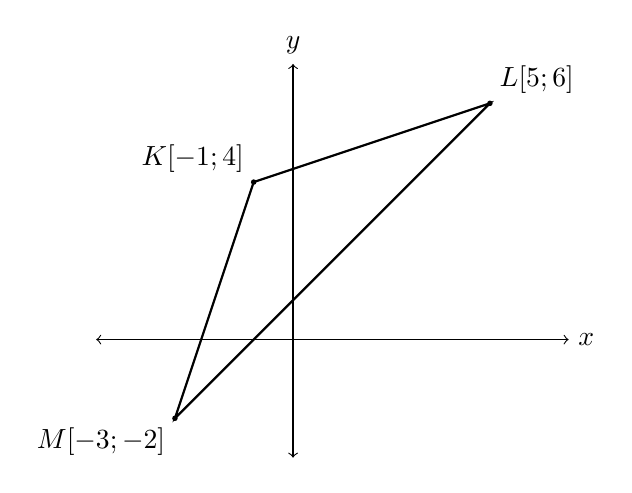
\begin{tikzpicture}[scale=0.5]

            % Body trojúhelníku
            \coordinate (K) at (-1,4);
            \coordinate (L) at (5,6);
            \coordinate (M) at (-3,-2);

            % Osy x a y
            \draw[<->] (-5,0) -- (7,0) node[right] {$x$};
            \draw[<->] (0,-3) -- (0,7) node[above] {$y$};

            % Trojúhelník
            \draw[thick] (K) -- (L) -- (M) -- cycle;

            % Body K, L, M
            \fill (K) circle (2pt) node[above left] {$K[-1;4]$};
            \fill (L) circle (2pt) node[above right] {$L[5;6]$};
            \fill (M) circle (2pt) node[below left] {$M[-3;-2]$};
        \end{tikzpicture}
        \caption{Trojúhelník $KLM$}
        \label{fig:Parametric_lines_in_triangle}
    \end{figure}

    \begin{enumerate}[label=\alph*), leftmargin=2em]

        \item \textbf{Přímka, na níž leží strana $LM$}

        Přímka obsahující stranu $LM$ prochází body $L[5;6]$ a
        $M[-3;-2]$. Její směrový vektor můžeme určit jako
        \[
            \overrightarrow{LM}
            =
            (-3-5;-2-6)
            =
            (-8;-8).
        \]

        Protože směrový vektor přímky můžeme nahradit jeho libovolným nenulovým násobkem, můžeme použít jednodušší vektor
        \[
            \vec{u}_{LM}=(-1;-1).
        \]

        Přímka prochází například bodem $L[5;6]$, a proto její
        parametrické vyjádření je
        \begin{align*}
            p_{LM}: x &= 5-t,\\
                    y &= 6-t;
                    \quad t\in\mathbb{R}.
        \end{align*}

        Správnost můžeme ověřit zjištěním, zda bod $M[-3;-2]$ leží na přímce $p_{LM}$.
        Dosazením do parametrického vyjádření získáme
        \begin{align*}
            -3 &= 5-t,\\
            -2 &= 6-t.
        \end{align*}
        Po upravení obou rovnic dostáváme
        \begin{align*}
            t &= 5+3=8,\\
            t &= 6+2=8.
        \end{align*}
        Odtud $t=8$, což potvrzuje, že bod $M$ leží na přímce $p_{LM}$.
        Přímka $p_{LM}$ obsahující stranu $LM$ je znázorněna na obrázku \ref{fig:Triangle_line_LM}.

        \begin{figure}[H]
            \centering
            \begin{tikzpicture}[scale=0.5]
            
                % Body trojúhelníku
                \coordinate (K) at (-1,4);
                \coordinate (L) at (5,6);
                \coordinate (M) at (-3,-2);
            
                % Osy
                \draw[<->] (-5,0) -- (7,0) node[right] {$x$};
                \draw[<->] (0,-4) -- (0,8) node[above] {$y$};
            
                % Trojúhelník
                \draw[thin,dashed] (K) -- (L) -- (M) -- cycle;
            
                % Přímka obsahující stranu LM
                \draw[thick] (-5,-4) -- (7,8)
                    node[right] {$p_{LM}$};
            
                % Směrový vektor
                \draw[vector] (L) -- ($(L)!0.4!(M)$)
                    node[midway, below left, sloped] {$\vec{u}_{LM}$};
            
                % Body
                \fill (K) circle (2pt) node[above left] {$K$};
                \fill (L) circle (2pt) node[above left] {$L$};
                \fill (M) circle (2pt) node[below right] {$M$};
            
            \end{tikzpicture}
            \caption{Přímka $p_{LM}$, na níž leží strana $LM$ trojúhelníku $KLM$.}
            \label{fig:Triangle_line_LM}
        \end{figure}

        \item \textbf{Výška $v_m$ vedená z vrcholu $M$}

        Výška $v_m$ prochází vrcholem $M$ a je kolmá ke straně $KL$.
        Nejprve proto určíme směrový vektor přímky obsahující stranu
        $KL$:
        \[
            \overrightarrow{KL}
            =
            (5-(-1);6-4)
            =
            (6;2).
        \]

        Tento vektor můžeme zjednodušit na
        \[
            \vec{u}_{KL}=(3;1).
        \]

        Směrový vektor výšky musí být k vektoru $\vec{u}_{KL}$ kolmý, využijeme vlastnost kolmosti vektorů (viz větu o kolmosti vektorů \ref{def:Fast_orthogonal_vector}).
        Zvolíme například
        \[
            \vec{u}_{v_m}=(1;-3),
        \]

        Výška $v_m$ prochází bodem $M[-3;-2]$ a má směrový vektor $\vec{u}_{v_m}$, a proto její parametrické
        vyjádření je
        \begin{align*}
            v_m: x &= -3+t,\\
                 y &= -2-3t;
                 \quad t\in\mathbb{R}.
        \end{align*}

        Výška $v_m$ vedená z vrcholu $M$ kolmo k přímce obsahující stranu $KL$ je znázorněna na obrázku \ref{fig:Triangle_altitude_vm}.

        \begin{figure}[H]
            \centering
            \begin{tikzpicture}[scale=0.5]
            
                % Body trojúhelníku
                \coordinate (K) at (-1,4);
                \coordinate (L) at (5,6);
                \coordinate (M) at (-3,-2);
            
                % Pata výšky na přímce KL
                \coordinate (P) at (-4.6,2.8);
            
                % Osy
                \draw[<->] (-6,0) -- (7,0) node[right] {$x$};
                \draw[<->] (0,-5) -- (0,8) node[above] {$y$};
            
                % Trojúhelník
                \draw[thin,dashed] (K) -- (L) -- (M) -- cycle;
            
                % Přímka obsahující stranu KL
                \draw[thin] (-6,2.33) -- (7,6.67);
            
                % Výška vm
                \draw[very thick] (-5.5,5.5) -- (-1.5,-6.5)
                    node[right] {$v_m$};
            
                % Pravý úhel
                \draw
                    ($(P)+(0.267,0.083)$)
                    --
                    ($(P)+(0.183,0.333)$)
                    --
                    ($(P)+(-0.1,0.25)$);
            
                % Body
                \fill (K) circle (2pt) node[above left] {$K$};
                \fill (L) circle (2pt) node[above right] {$L$};
                \fill (M) circle (2pt) node[below right] {$M$};
                \fill (P) circle (1.5pt) node[above left] {$P$};
            
            \end{tikzpicture}
            \caption{Výška $v_m$ prochází vrcholem $M$ a je kolmá k přímce obsahující stranu $KL$.}
            \label{fig:Triangle_altitude_vm}
        \end{figure}

        \item \textbf{Osa strany $KL$}

        Osa strany $KL$ prochází jejím středem a je ke straně $KL$ kolmá. Nejprve určíme střed strany:
        \begin{align*}
            S_{KL}
            &=
            \left[
                \frac{-1+5}{2};
                \frac{4+6}{2}
            \right]
            =
            [2;5].
        \end{align*}

        Protože osa strany $KL$ je ke straně $KL$ kolmá, můžeme jako
        její směrový vektor použít stejný vektor jako u výšky $v_m$:
        \[
            \vec{u}_{o_{KL}} = \vec{u}_{v_m} = (1;-3).
        \]

        Parametrické vyjádření osy strany $KL$ je tedy
        \begin{align*}
            o_{KL}: x &= 2+t,\\
                    y &= 5-3t;
                    \quad t\in\mathbb{R}.
        \end{align*}

        Výška $v_m$ a osa strany $KL$ mají stejné směrové vektory,
        a jsou proto navzájem rovnoběžné, což odpovídá skutečnosti,
        že obě přímky jsou kolmé ke straně $KL$.

        Osa strany $KL$ je znázorněna na obrázku \ref{fig:Triangle_perpendicular_bisector_KL}. 
        Prochází středem $S_{KL}$ a je ke straně $KL$ kolmá.

        \begin{figure}[H]
            \centering
            \begin{tikzpicture}[scale=0.5]

                % Body trojúhelníku
                \coordinate (K) at (-1,4);
                \coordinate (L) at (5,6);
                \coordinate (M) at (-3,-2);
                \coordinate (Skl) at (2,5);

                % Osy
                \draw[<->] (-5,0) -- (7,0) node[right] {$x$};
                \draw[<->] (0,-4) -- (0,9) node[above] {$y$};

                % Trojúhelník
                \draw[thin,dashed] (K) -- (L) -- (M) -- cycle;

                % Zvýraznění strany KL
                \draw[thin] (K) -- (L);

                % Osa strany KL
                \draw[very thick] (0.5,9.5) -- (4.5,-2.5)
                    node[below right] {$o_{KL}$};

                % Pravý úhel ve středu strany
                \draw
                        ($(Skl)+(0.267,0.083)$)
                        --
                        ($(Skl)+(0.183,0.333)$)
                        --
                        ($(Skl)+(-0.1,0.25)$);

                % Body
                \fill (K) circle (2pt) node[above left] {$K$};
                \fill (L) circle (2pt) node[above right] {$L$};
                \fill (M) circle (2pt) node[below left] {$M$};
                \fill (Skl) circle (2pt) node[above left] {$S_{KL}$};

            \end{tikzpicture}
            \caption{Osa strany $KL$ prochází jejím středem $S_{KL}$ a je ke straně $KL$ kolmá.}
            \label{fig:Triangle_perpendicular_bisector_KL}
        \end{figure}

        \item \textbf{Těžnice $t_L$ vedená z vrcholu $L$}

        Těžnice $t_L$ spojuje vrchol $L$ se středem protější strany
        $KM$. Nejprve proto určíme střed strany $KM$:
        \begin{align*}
            S_{KM}
            &=
            \left[
                \frac{-1+(-3)}{2};
                \frac{4+(-2)}{2}
            \right]
            =
            [-2;1].
        \end{align*}

        Směrový vektor těžnice získáme jako vektor směřující z bodu
        $L$ do bodu $S_{KM}$:
        \[
            \overrightarrow{LS_{KM}}
            =
            (-2-5;1-6)
            =
            (-7;-5).
        \]

        Těžnice prochází bodem $L[5;6]$, a proto její parametrické
        vyjádření je
        \begin{align*}
            t_L: x &= 5-7t,\\
                 y &= 6-5t;
                 \quad t\in\mathbb{R}.
        \end{align*}

        Těžnice $t_l$ spojující vrchol $L$ se středem $S_{KM}$ protější strany je znázorněna na obrázku \ref{fig:Triangle_median_tl}.

        \begin{figure}[H]
            \centering
            \begin{tikzpicture}[scale=0.5]
            
                % Body trojúhelníku
                \coordinate (K) at (-1,4);
                \coordinate (L) at (5,6);
                \coordinate (M) at (-3,-2);
                \coordinate (Skm) at (-2,1);
            
                % Osy
                \draw[<->] (-5,0) -- (7,0) node[right] {$x$};
                \draw[<->] (0,-4) -- (0,8) node[above] {$y$};
            
                % Trojúhelník
                \draw[thin,dashed] (K) -- (L) -- (M) -- cycle;
            
                % Těžnice
                \draw[thin] (6.4,7) -- (-4.8,-1)
                    node[below left] {$t_l$};
            
                % Zvýraznění úseku od L do středu
                \draw[very thick] (L) -- (Skm);
            
                % Body
                \fill (K) circle (2pt) node[above left] {$K$};
                \fill (L) circle (2pt) node[right] {$L$};
                \fill (M) circle (2pt) node[below left] {$M$};
                \fill (Skm) circle (2pt) node[above left] {$S_{KM}$};
            
            \end{tikzpicture}
            \caption{Těžnice $t_l$ vedená z vrcholu $L$ do středu $S_{KM}$ protější strany.}
            \label{fig:Triangle_median_tl}
        \end{figure}

        \item \textbf{Střední příčka $S_{KL}S_{KM}$}

        Střední příčka spojuje středy dvou stran trojúhelníku.
        V předchozích částech jsme určili
        \[
            S_{KL}=[2;5],
            \qquad
            S_{KM}=[-2;1].
        \]

        Směrový vektor přímky obsahující střední příčku je
        \[
            \overrightarrow{S_{KL}S_{KM}}
            =
            (-2-2;1-5)
            =
            (-4;-4).
        \]

        Tento vektor můžeme nahradit jednodušším směrovým vektorem
        \[
            \vec{u}_s=(-1;-1).
        \]

        Parametrické vyjádření přímky obsahující střední příčku je
        proto
        \begin{align*}
            s: x &= 2-t,\\
               y &= 5-t;
               \quad t\in\mathbb{R}.
        \end{align*}

        Směrový vektor střední příčky je rovnoběžný se směrovým
        vektorem strany $LM$, protože
        \[
            \overrightarrow{LM}=(-8;-8)
            =
            8(-1;-1).
        \]
        Tím se potvrzuje známá vlastnost střední příčky trojúhelníku:
        \[
            S_{KL}S_{KM}\parallel LM.
        \]

        Střední příčka $S_{KL}S_{KM}$ je znázorněna na obrázku \ref{fig:Triangle_midline}.
        Z obrázku je patrné, že je rovnoběžná se stranou $LM$.

        \begin{figure}[H]
            \centering
            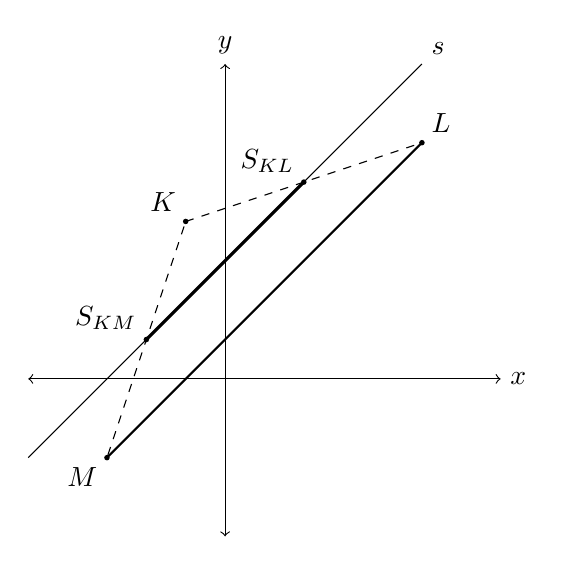
\begin{tikzpicture}[scale=0.5]
            
                % Body trojúhelníku
                \coordinate (K) at (-1,4);
                \coordinate (L) at (5,6);
                \coordinate (M) at (-3,-2);
                \coordinate (Skl) at (2,5);
                \coordinate (Skm) at (-2,1);
            
                % Osy
                \draw[<->] (-5,0) -- (7,0) node[right] {$x$};
                \draw[<->] (0,-4) -- (0,8) node[above] {$y$};
            
                % Trojúhelník
                \draw[thin,dashed] (K) -- (L) -- (M) -- cycle;
            
                % Strana LM
                \draw[thick] (L) -- (M);
            
                % Přímka obsahující střední příčku
                \draw[thin] (-5,-2) -- (5,8)
                    node[above right] {$s$};
            
                % Střední příčka
                \draw[very thick] (Skl) -- (Skm);
            
                % Body
                \fill (K) circle (2pt) node[above left] {$K$};
                \fill (L) circle (2pt) node[above right] {$L$};
                \fill (M) circle (2pt) node[below left] {$M$};
                \fill (Skl) circle (2pt) node[above left] {$S_{KL}$};
                \fill (Skm) circle (2pt) node[above left] {$S_{KM}$};
            
            \end{tikzpicture}
            \caption{Střední příčka $S_{KL}S_{KM}$ je rovnoběžná se stranou $LM$.}
            \label{fig:Triangle_midline}
        \end{figure}
    \end{enumerate}
\end{example}
